%
\section{Automatische Statische Analyse}
Zur statischen Analyse von C\# Programmen stehen eine Reihen an Werkzeugen zur Verfügung. Einerseits gibt es in die Entwicklungsumgebung integrierte Werkzeuge wie \emph{NDepend}, \emph{ReSharper} und das von Visual Studio bereitgestellt Tool, andererseits eigenständige Programme wie \emph{Gendarme} und \emph{SourceMonitor}.

\subsection{NDepend}
\emph{NDepend} führt statischen Analysen von Projekten durch, erstellt dabei Softwarelandkarten, Codemetriken und überprüft ob Quelltextregel eingehalten werden.~\cite{ndepend} Auf der \enquote{Dashboard} genannten Übersicht erstellt NDepend eine Zusammenfassung aller Analysen. 

\subsubsection{Quelltextregel}
NDepend ermittelt in C\# Essentials insgesamt 37 verletzte Regeln, dabei finden 150 Regeln Anwendung. An dieser Stelle soll nur auf die als kritisch markierten Regeln eingegangen werden. 3 kritische Regelverletzungen ermittelt NDepend: Methods too complex (2), Potenially dead Methods (6), Potentially dead Types (6). Weitere verletzte Regeln sind in erster Linie nicht eingehaltene Namenskonventionen, Sichtbarkeiten und Design Schwächen. Um potentielle Fehler zu finden, werden im Folgenden kritische Stellen genauer analysiert.

\paragraph{Methods too complex}

\paragraph{Potentially dead Methods} In C\# Essentials findet NDepend sechs mögliche Stellen, an denen Quelltext nicht ausgeführt wird. In Abbildung~\ref{fig:dead-methods} sieht man zwei der gefundenen Stellen. Bei allen handelt es sich um nicht aufgerufenen Konstruktoren. Jedoch handelt es sich bei den gefundenen Stellen um keine Konstruktoren. Ähnlich der MoveNext Methode diagnostiziert eine falsche Methode an der richtigen Stelle. %TODO: versuche rauszufinden, welche Ursache hier vorliegt.

\begin{figure}[ht]
\centering
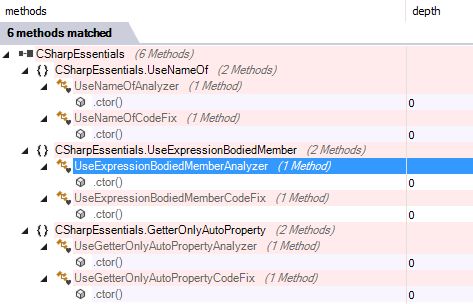
\includegraphics[width=0.8\textwidth]{images/dead-methods.png}
\caption{Potentially dead Methods}
\vspace{0.1cm}
Von NDepend gefundener wahrscheinlich nicht aufgerufener Quelltext
\label{fig:dead-methods}
\end{figure}

\subsubsection{Quelltextmetriken}
Mit Hilfe des \enquote{Code Metrics View} visualisiert \emph{NDepend} Quelltextmetriken. Auflösungen von Assembly über Namespaces bis Methoden stehen zur Auswahl. In größeren System, welche aus mehren Assemblies bestehen, möchte man nach kritischen Teilprogrammen suchen. Mit knapp über 1000 Quelltextzeilen und nur einer Assembly in CSharpEssentials ist die Auflösung nach Methoden am sinnvollsten. IL Nesting Depth, Cyclomatic Complexity und IL Cyclomatic Complexity erzeugen die in den Abbildungen~\ref{fig:nd-il-nesting-depth},~\ref{fig:nd-cyclomatic-complexity} und ~\ref{fig:nd-il-cyclomatic-complexity} dargestellten Code Metric Views. Metriken mit einem führenden \enquote{IL} werden auf Basis der \enquote{Intermediate Language} erstellt. Mehr zur \emph{IL} in Abschnitt \ref{sec:gendarme}. Die Programmierer von NDepend definieren jede Metrik und geben zusätzlich einen empfohlenen Maximalwert an.~\cite{ndepend-metrics}

\begin{figure}[ht]
	\centering
	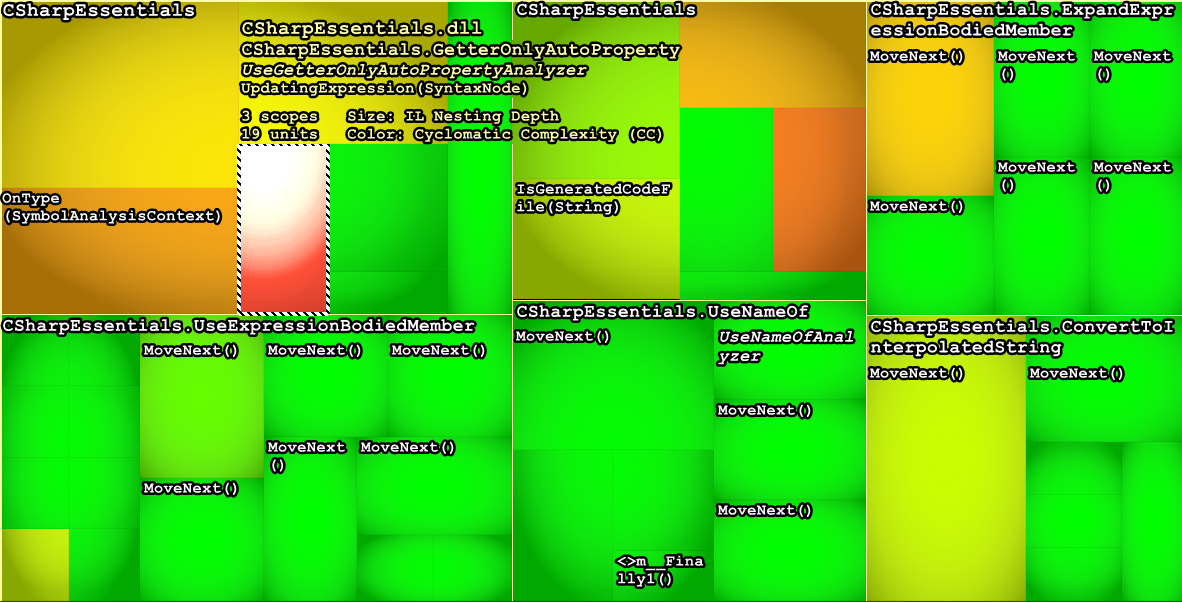
\includegraphics[width=0.8\textwidth]{images/nd-il-nesting-depth.png}
	\caption{}
	\vspace{0.1cm}
	\label{fig:nd-il-nesting-depth}
\end{figure}

\begin{figure}[ht]
	\centering
	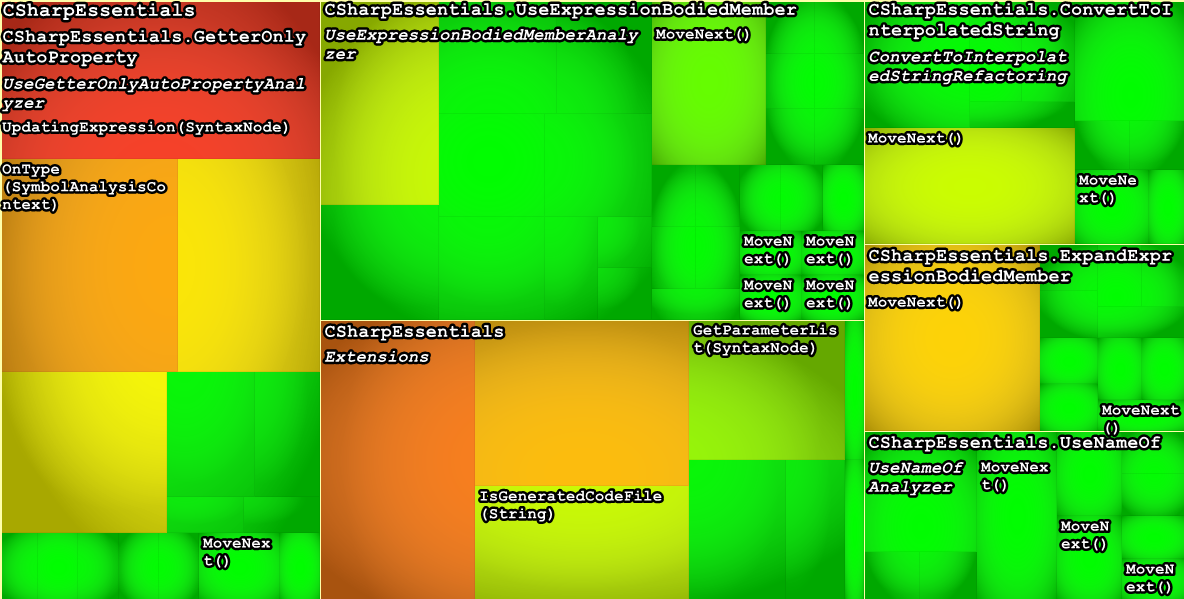
\includegraphics[width=0.8\textwidth]{images/nd-cyclomatic-complexity.png}
	\caption{}
	\vspace{0.1cm}
	\label{fig:nd-cyclomatic-complexity}
\end{figure}

\begin{figure}[ht]
	\centering
	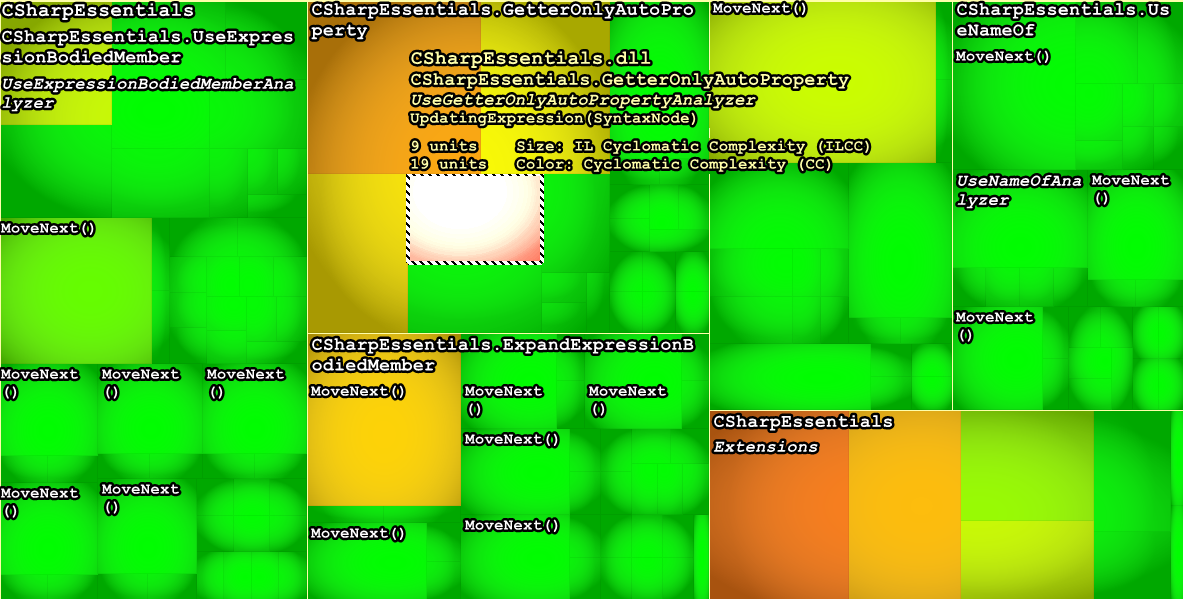
\includegraphics[width=0.8\textwidth]{images/nd-il-cyclomatic-complexity.png}
	\caption{}
	\vspace{0.1cm}
	\label{fig:nd-il-cyclomatic-complexity}
\end{figure}

\subsection{ReSharper}
Mit \emph{ReSharper} bietet JetBrains ein Werkzeug zur statischen Analyse für Visual Studio an.~\cite{resharper} 

\subsection{Visual Studio Tools}
Visual Studio analysiert Code, erstellt dabei Quelltextmetriken und kann zum Beispiel Code-Clone identifizieren.

\subsubsection{Quelltextmetriken}

\subsubsection{Code-Clone}


\subsection{Gendarme}
\label{sec:gendarme}
Gendarme analysiert Programme und Bibliotheken, welche in den verschiedenen .NET Sprachen geschrieben wurden. Dafür benötigt Gendarme eine kompilierte Assembly, weil es nicht den C\# statisch analysiert, sondern ein daraus erzeugte Spracheformat: Das ECMA CIL~\footnote{European Computer Manufacturers Association Common Language Infrastructure} Format.~\cite{ecma} Die CIL wird mit Hilfe von der Bibliothek Cecil analysiert.~\cite{cecil} Gendarme generiert auf Basis dieser Analyse Berichte. Sie können als HTML-Datei exportiert werden.

\paragraph{ECMA CIL}

\subsubsection{Fehler}

\subsubsection{Sicherheiten}


\subsection{SourceMonitor}
Der Fokus von \emph{Source Monitor} liegt auf der Analyse von Quelltextmetriken. Es bietet die Möglichkeit einzelne 

\subsubsection{Kiviat-Chart}

\subsection{ASA Werkzeuge - Ein Vergleich}
Tools wie \emph{NDepend} und \emph{ReSharper} stellen eine große Menge an Funktionen bereit, welche die ASA von C\# Programmen und das Schreiben von Tests erleichtern. Die Fehler in den Analysen von \emph{NDepend} sind störend gewesen. Ein Werkzeug, welches für Preis ab 300 \euro ~erhältlich ist, muss eine deutlich bessere Ergebnisqualität bereitstellen. Die spezialisierten Programme \emph{Gendarme} und \emph{SourceMonitor} sind erheblich übersichtlicher als die Visual Studio Erweiterungen. Mit \emph{Gendarm} ist die Analyse deshalb besonderes einfach gewesen, weil die nötigen Einstellungen direkt vor der Analyse in einem einfachen Dialog konfiguriert werden. Jedoch sind die Ergebnisse weniger zufriedenstellend als die von zum Beispiel \emph{NDepend}, weil die Verbesserungsvorschläge keine direkten Probleme im Quelltext adressieren. Ein Besonderheit sind die Kiviat-Charts in \emph{Source Monitor}, da sie eine Form der graphischen Analyse von Quelltext ermöglichen, welche sonst kein anderes Werkzeug anbietet.
